\subsubsection{Trigonometrische Funktionen}
\vspace{3mm}
\begin{minipage}{0.4\linewidth}
    \begin{flalign}
        &\tan{\varphi} = \frac{\sin{\varphi}}{\cos{\varphi}}&\\
        &\cot{\varphi} = \frac{\cos{\varphi}}{\sin{\varphi}}&
    \end{flalign}
\end{minipage}
\hfill
\begin{minipage}{0.4\linewidth}
    \begin{flalign}
        &\sinh{x} = \frac{e^{x} − e^{−x}}{2}&\\
        &\cosh{x} = \frac{e^{x} + e^{−x}}{2}&\\
        &\tanh{x} = \frac{\sinh{x}}{\cosh{x}}&\\
        &\coth{x} = \frac{\cosh{x}}{\sinh{x}}&
    \end{flalign}
\end{minipage}

\begin{tabularx}{\linewidth}{|X|X|X|X|}
    \hline
    \textbf{Sin} & \textbf{Cos} & \textbf{Tan} & \textbf{Cot}\\
    \hline
    \textbf{G} & \textbf{A} & \textbf{G} & \textbf{A}\\
    \hline
    \textbf{H} & \textbf{H} & \textbf{A} & \textbf{G}\\
    \hline
\end{tabularx}

\begin{minipage}{0.29\linewidth}
    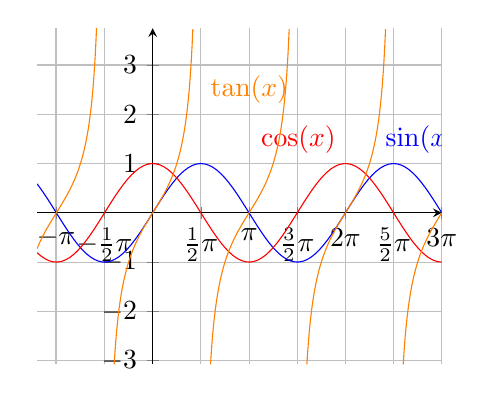
\begin{tikzpicture}
    \begin{axis}[enlargelimits=false,
                 axis lines=middle,
                 scale=0.75,
                 xtick={-3.15159, -1.57080, 0,
                         1.57080,  3.15159, 4.71239,
                         6.28318,  7.85398, 9.42478 }, 
                 xticklabels={$-\pi$, $-\frac{1}{2}\pi$, 0,
                              $\frac{1}{2}\pi$, $\pi$, $\frac{3}{2}\pi$,
                              $2\pi$, $\frac{5}{2}\pi$, $3\pi$ },
                 ytick={-3,-2,-1,0,1,2,3},
                 grid=major, % only a grid on the defined ticks
                 samples=100 % number of points
                 ]
     
      % sin
      \addplot[blue,no marks,domain=-1.2*pi:3*pi]{sin(deg(x))}; % deg to convert radians
      \node[right=10pt,above] at (axis cs:5*pi/2,1){\color{blue}$\sin(x)$};
     
      % cos
      \addplot[red,no marks,domain=-1.2*pi:3*pi] {cos(deg(x))};
      \node[above left] at (axis cs:2*pi,1){\color{red}$\cos(x)$};
     
      % tan, multiple parts because of singularities
      \addplot[orange,no marks,domain=-1.2*pi:-0.583*pi, ]{tan(deg(x))};
      \addplot[orange,no marks,domain=-0.4*pi:5*pi/12,   ]{tan(deg(x))};
      \addplot[orange,no marks,domain=27*pi/45:17*pi/12, ]{tan(deg(x))};
      \addplot[orange,no marks,domain=1.6*pi:29*pi/12,   ]{tan(deg(x))};
      \addplot[orange,no marks,domain=2.6*pi:36*pi/12,   ]{tan(deg(x))};
      \node[right] at (axis cs:pi/2,2.5){\color{orange}$\tan(x)$};
     
    \end{axis}
    \end{tikzpicture}
\end{minipage}
\hfill
\begin{minipage}{0.39\linewidth}
    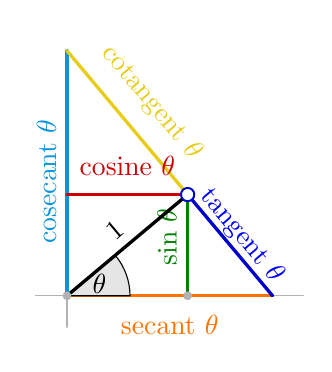
\begin{tikzpicture}[ 
        scale=2,  % Adjusts the overall size of the image line 
        cap=round, 
        line join=round, 
        very thick % Sets a default thickness for the lines 
        ] 
        
        % 1. Define colors to match the image 
        \colorlet{myred}{red!80!black} 
        \colorlet{mygreen}{green!50!black} 
        \colorlet{myblue}{blue!80!black} 
        \colorlet{myyellow}{yellow!80!orange!90!black} 
        \colorlet{myorange}{orange!90!red} 
        \colorlet{mylightblue}{cyan!80!blue} 
        \colorlet{mygray}{gray!60} 
        
        % 2. Define the angle (e.g., 40 degrees) 
        \def\th{40} 
        
        % 3. Define key coordinates based on the angle 
        \coordinate (O) at (0,0); 
        % Origin 
        \coordinate (P) at (\th:1); 
        
        % Point on the unit circle 
        \coordinate (P_on_x) at ({cos(\th)}, 0); 
        % Projection of P on the x-axis 
        \coordinate (P_on_y) at (0, {sin(\th)}); 
        % Projection of P on the y-axis 
        \coordinate (Sec_int) at ({1/cos(\th)}, 0); 
        % Intersection for the secant on the x-axis 
        \coordinate (Csc_int) at (0, {1/sin(\th)}); 
        % Intersection for the cosecant on the y-axis 
        
        
        % 4. Draw the elements in a specific order (from back to front) 
        % Axes (thin gray lines) 
        \draw[mygray, thin] (-0.2,0) -- (1.5,0); 
        \draw[mygray, thin] (0,-0.2) -- (0,1.5); 
        
        % The Cosecant and Secant axis lines 
        
        % Cosecant line (light blue) 
        \draw[mylightblue] (O) -- (Csc_int) node[midway, above, sloped, mylightblue, xshift=-3pt] {cosecant $\theta$}; 
        
        % Secant line (orange) 
        \draw[myorange] (O) -- (Sec_int) node[midway, below, myorange, yshift=-3pt] {secant $\theta$}; 
        
        % Unit Circle (thin gray line) 
        % \draw[mygray, thin] (O) circle (1); 
        
        % Angle theta representation $
        \draw[fill=gray!20, draw=black, thin, line width=0.4pt] (O) -- (0.4,0) arc (0:\th:0.4) -- cycle; 
        \node at (\th/2:0.22) {$\theta$}; 
        
        % The Cotangent and Tangent hypotenuse lines 
        % Cotangent line (yellow) 
        \draw[myyellow] (P) -- (Csc_int) node[midway, above, sloped, myyellow, yshift=3pt] {cotangent $\theta$}; 
        
        % Tangent line (blue) 
        \draw[myblue] (P) -- (Sec_int) node[midway, above, sloped, blue, yshift=-3pt] {tangent $\theta$}; 
        
        % The Sine and Cosine lines 
        % Sine line (green) 
        \draw[mygreen] (P_on_x) -- (P) node[midway, above, sloped, mygreen, xshift=3pt] {sin $\theta$}; 
        
        % Cosine line (red) $
        \draw[myred] (P_on_y) -- (P) node[midway, above, myred, yshift=3pt] {cosine $\theta$}; 
        
        % Radius line (black) 
        \draw (O) -- (P) node[midway, above, sloped, black] {1}; 
        
        % 5. Draw the points on top 
        \fill[mygray] (O) circle (0.8pt); 
        
        % Point at origin 
        \fill[mygray] (P_on_x) circle (0.8pt); 
        
        % Point for sine on x-axis 
        % Point on the circle (blue ring with white fill) 
        \draw[myblue, fill=white, line width=0.7pt] (P) circle (1.2pt); 
    \end{tikzpicture}
\end{minipage}



